%!TEX root = ../thesis.tex

\chapter{Technologies}\label{chapter:technologies}


% TODO mettere da qualche parte overview of underlaying network technologies
% Hardware Addressing Schemes
	
	This chapter explains more in detail the underlying technologies of this project.
	
	Starting from the general definition of a network and the most common architectures, to radio technologies work and then micro-controllers.
	

%	In this chapter we describe DTNs, the notion of peer-to-peer and overlay networks.
%	
%	internetworking \cite{internetworking}
	
	
% TODO andare a recuperare dal libro di douglas
\section{Approaches To Network Communication}
	
	\begin{center}
		\begin{minipage}[H]{0.9\columnwidth}
			\begin{center}
				``\textit{A computer network is a structure that makes available to a data processing user at one place some data processing function or service performed at another place.}''~\cite{nla.cat-vn252493}
			\end{center}
		\end{minipage}
	\end{center}
	
	% - % - % - % - % - % - % - % - % - % - % - % - % - % - % - % - 
	
	Given the definition of computer network by Paul E. Green, it is easy to understand its importance in today's society. % TODO ARGOMENTARE
	
	unavoidable in our daily life
	
	Il fatto che tutti abbiano accesso ad internet non solo ha permesso cambiamenti a livello culturale ma anche nel mercato economico
	
	In alcuni paesi l'importanza di dare accesso a questa rete è riconosciuta per legge
	
	Da non confondere Internet con internet
	
	% - % - % - % - % - % - % - % - % - % - % - % - % - % - % - % - 	

	% http://www.redbooks.ibm.com/abstracts/gg243376.html
	A network of networks is called internetwork, shortened by internet; however, the Internet, with a capital I, is a set of worldwide interconnected networks \cite{gg243376}.
	
	Questa distinzione è stata cominciata ad essere fatta / proposta in the beginning of the 1980s\footnote{\href{https://datatracker.ietf.org/doc/html/rfc871}{RFC 871 (1982): A PERSPECTIVE ON THE ARPANET REFERENCE MODEL}}$^{,}$\footnote{\href{https://datatracker.ietf.org/doc/html/rfc872}{RFC 872 (1982): TCP-ON-A-LAN}}, when computers were becoming more and more accessible not only to to companies and universities, but also in households with the advent of MS-DOS\footnote{\href{https://github.com/microsoft/MS-DOS}{MS-DOS source code on GitHub}}, thus ARPANET was expanding and LANs were not enough anymore to accomodate the amount of data travelling from one place to another.
	
	from the 1980s, As described in \cite{gg243376}, it is possible to divide the Internet such as the following groups of networks:
	\begin{itemize}[noitemsep]
		\item Backbones: Large networks that exist primarily to interconnect other networks. Also known as network access points (NAPs) or Internet Exchange
		\item Regional networks connecting, for example, universities and colleges.
		\item Commercial networks providing access to the backbones to subscribers, and networks owned by commercial organizations for internal use that also have connections to the Internet.
		\item Local networks, such as campus-wide university networks
	\end{itemize}

	% Inserire immagina backbone, ecc

	Thus came the need for a better structure that could organize at best these components in a more robust, but also flexible, large network.
	
	% inserire immagine con la nuvoletta che si vede dentro e non si vede dentro
	
	% distinzione tra distributed systems e computer network
	
	It is important to understand the difference between network architecture and network topology.
	
	A network architecture, as described by by Paul E. Green, ``is a complete definition of all the layers necessary to build the network''\cite{nla.cat-vn252493}.
	This is focused on the network software, which needs to be highly structure in order to allow for heterogeneous systems to communicate with each other.
	One example of network architecture is the ISO/OSI reference model, which is implemented by the TCP/IP stack of protocols.
	% Inserire immagine tcp/ip vs iso/osi vedi tenenbaum pag 42
	``A protocol is a set of agreements for interaction of two or more parties and is expressed by three components, syntax (e.g., a set of headers, a set of commands/responses), semantics (the actions and reactions that take place, including the exchange of messages), and timing, the sequencing and concurrency aspects of the protocol.''\cite{nla.cat-vn252493}.
	Different types of network use different architectures, based on the transmission medium and how well this performs (errors, speed, etc.)
	
	% https://www.omnisci.com/technical-glossary/network-topology
	On the other hand, the network topology refers to the manner in which the links and nodes of a network are arranged to relate to each other.
	
	% inserire immagine con le varie architetture di rete	
	
	\begin{figure}[h!]
		\centering
		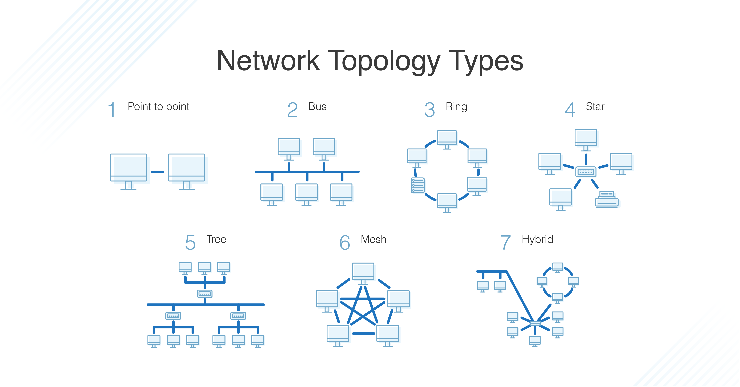
\includegraphics[width=\textwidth-4cm]{resources/img/chap3/network_topologies.png}
		\caption{Diagrammatic view of the Universal Product Code}
		\label{fig:upc_patent}
	\end{figure}
	
	% COPIATO DA INTERNET: responsible for technical management of IETF activities and the Internet standards process
	Nowadays, the organization responsible for technical management of IETF activities and the Internet standards process is the Internet Engineering Steering Group (IESG)\footnote{\url{https://www.ietf.org/about/groups/iesg/}}.
	It is necessary to have an organization looking over the Internet itself since it gives the regulations that allow all devices to interconnect with each other.
		
	Networks can be categorized based on their span.
	Instead, vendors apply the terms loosely to help customers distinguish among technologies.
	\begin{itemize}
		\item WAN: WAN technologies, sometimes called long haul networks, provide communication
		over long distances.
		\item MAN
		\item LAN: 	LAN technologies provide the highest speed connections among computers, but
		sacrifice the ability to span long distances.
		\item PAN
	\end{itemize}
	
	
	\newpage	

\section{Radio technologies}\label{sec:section_two}
	
	In order to give a complete picture of radio transmitting technologies, it is important to make a distinction among the ones that are made for internal or nearby use vs the ones that are used for longer distances.
	
	% TODO spiegare LAN, MAN, WAN
	
	With new transmission technologies, new network architectures have emerged
	
	% TODO spiegare LPWAN
	
	Distinction of low cost vs higher cost
	% http://iotfactory.eu/iot-knowledge-center/overview-of-iot-networks/
	
	\begin{figure}
		\centering
		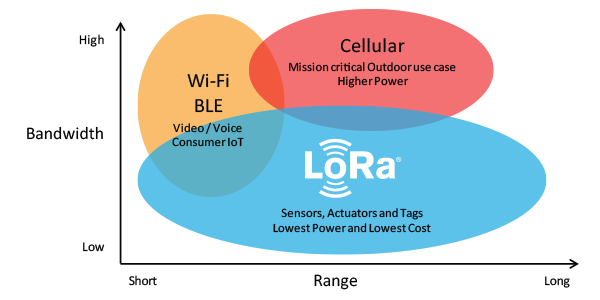
\includegraphics[width=\textwidth]{resources/img/LoRa_Why_Range}
		\caption{}
	\end{figure}
	
	% PAPER : LPWAN Technologies: Emerging ApplicationCharacteristics, Requirements, andDesign Considerations
	\begin{figure}
		\centering
		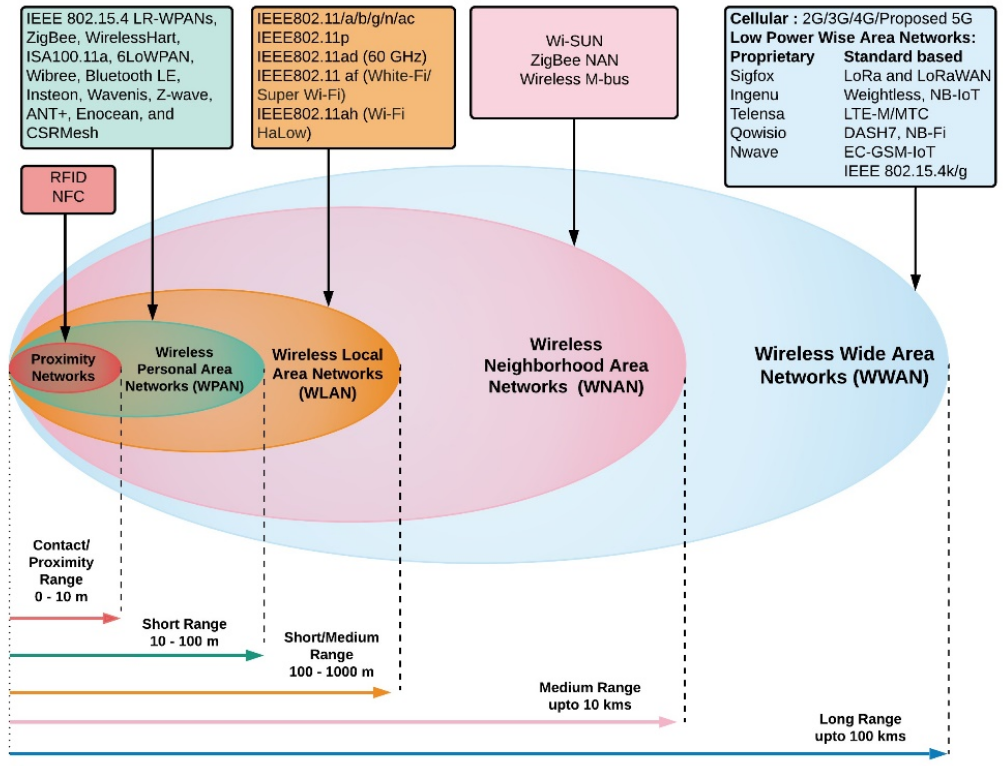
\includegraphics[height=\textwidth, angle=90]{resources/img/iot_range}
		\caption{}
	\end{figure}
	
	\subsection{LoRa}
	
		https://lora-alliance.org/
		
		https://www.semtech.com/lora

	\subsection{LoRaWAN}
	
	\subsection{Bluetooth}		
	
	\subsection{WiFi}



	IEEE 802.11, better known in the public as WiFi, short for wireless fidelity
	
	\subsection{LTE}
	


\section{LoRa and LoRaWAN}

\section{Hardware (Microcontrollers)}

	Microcontrollers (or MCUs) are compact integrated circuits designed to govern a specific operation in an embedded system.
	
	Devices and CPUs have become smaller and more granular, allowing to have simple micro computers that need very little power resources, both computational and battery, that they can be used for very specific functions.
	
	Some examples can be:
	\begin{itemize}
		\item smog detector, which sounds an alarm when excess smog is sensed
		\item car range detector, that sends an alarm to the car's braking system when there is an object in front of it
		\item etc.
	\end{itemize}

	\subsection{Arduino}
	
		% https://www.arduino.cc/en/Main/AboutUs
		
	
	\subsection{Raspberry Pi}
		
		\noindent
		\begin{minipage}{0.5\textwidth}% adapt widths of minipages to your needs
			
\includegraphics[width=\textwidth]{resources/img/51-513503_pi-raspberry-pi-logo}
			\captionof{figure}{\textit{Pycom} company logo}
		\end{minipage}%
		\hfill%
		\begin{minipage}{0.55\textwidth}\raggedright
			Yesterday,\\
			all my troubles seemed so far away\\
			Now it looks as though they're here to stay\\
			Oh, I believe in yesterday.				Yesterday,\\
			all my troubles seemed so far away\\
			Now it looks as though they're here to stay\\
		\end{minipage}	
		
		\subsection{Pycom}
	
		\noindent
		\begin{minipage}{0.5\textwidth}% adapt widths of minipages to your needs
			
\includegraphics[width=\textwidth]{resources/img/pycom-logo-new-rp1}
			\captionof{figure}{\textit{Pycom} company logo}
		\end{minipage}%
		\hfill%
		\begin{minipage}{0.55\textwidth}\raggedright
			Yesterday,\\
			all my troubles seemed so far away\\
			Now it looks as though they're here to stay\\
			Oh, I believe in yesterday.				Yesterday,\\
			all my troubles seemed so far away\\
			Now it looks as though they're here to stay\\
		\end{minipage}
		
		A Pycom development board has considerably more I/O than a standard Arduino, but probably comparable to an Arduino Mega. Easy to program via Python. Good example code from Pycom. Small community. Low cost. Not at all comparable to Raspberry Pi in terms of software flexibility.
		
		% https://www.reddit.com/r/IOT/comments/kx6knr/what_do_people_think_of_pycom_products/
		A complete LoRa gateway (Pygate + WiPy + IP67 box + antenna) costs around \$100, which is pretty good. So far very stable, and it was easy to configure. There's a PoE unit, but I use WiFi (at my home).
		
% TODO ADD TO REFERENCES
% https://docs.pycom.io/gitbook/assets/lopy4-pinout.pdf
